% Options for packages loaded elsewhere
\PassOptionsToPackage{unicode}{hyperref}
\PassOptionsToPackage{hyphens}{url}
%
\documentclass[
]{article}
\usepackage{amsmath,amssymb}
\usepackage{lmodern}
\usepackage{ifxetex,ifluatex}
\ifnum 0\ifxetex 1\fi\ifluatex 1\fi=0 % if pdftex
  \usepackage[T1]{fontenc}
  \usepackage[utf8]{inputenc}
  \usepackage{textcomp} % provide euro and other symbols
\else % if luatex or xetex
  \usepackage{unicode-math}
  \defaultfontfeatures{Scale=MatchLowercase}
  \defaultfontfeatures[\rmfamily]{Ligatures=TeX,Scale=1}
\fi
% Use upquote if available, for straight quotes in verbatim environments
\IfFileExists{upquote.sty}{\usepackage{upquote}}{}
\IfFileExists{microtype.sty}{% use microtype if available
  \usepackage[]{microtype}
  \UseMicrotypeSet[protrusion]{basicmath} % disable protrusion for tt fonts
}{}
\makeatletter
\@ifundefined{KOMAClassName}{% if non-KOMA class
  \IfFileExists{parskip.sty}{%
    \usepackage{parskip}
  }{% else
    \setlength{\parindent}{0pt}
    \setlength{\parskip}{6pt plus 2pt minus 1pt}}
}{% if KOMA class
  \KOMAoptions{parskip=half}}
\makeatother
\usepackage{xcolor}
\IfFileExists{xurl.sty}{\usepackage{xurl}}{} % add URL line breaks if available
\IfFileExists{bookmark.sty}{\usepackage{bookmark}}{\usepackage{hyperref}}
\hypersetup{
  pdftitle={Teaching Data Science to Students in Biology using R, RStudio and Learnr: Analysis of Three Years Data},
  hidelinks,
  pdfcreator={LaTeX via pandoc}}
\urlstyle{same} % disable monospaced font for URLs
\usepackage[margin=1in]{geometry}
\usepackage{longtable,booktabs,array}
\usepackage{calc} % for calculating minipage widths
% Correct order of tables after \paragraph or \subparagraph
\usepackage{etoolbox}
\makeatletter
\patchcmd\longtable{\par}{\if@noskipsec\mbox{}\fi\par}{}{}
\makeatother
% Allow footnotes in longtable head/foot
\IfFileExists{footnotehyper.sty}{\usepackage{footnotehyper}}{\usepackage{footnote}}
\makesavenoteenv{longtable}
\usepackage{graphicx}
\makeatletter
\def\maxwidth{\ifdim\Gin@nat@width>\linewidth\linewidth\else\Gin@nat@width\fi}
\def\maxheight{\ifdim\Gin@nat@height>\textheight\textheight\else\Gin@nat@height\fi}
\makeatother
% Scale images if necessary, so that they will not overflow the page
% margins by default, and it is still possible to overwrite the defaults
% using explicit options in \includegraphics[width, height, ...]{}
\setkeys{Gin}{width=\maxwidth,height=\maxheight,keepaspectratio}
% Set default figure placement to htbp
\makeatletter
\def\fps@figure{htbp}
\makeatother
\setlength{\emergencystretch}{3em} % prevent overfull lines
\providecommand{\tightlist}{%
  \setlength{\itemsep}{0pt}\setlength{\parskip}{0pt}}
\setcounter{secnumdepth}{5}
\ifluatex
  \usepackage{selnolig}  % disable illegal ligatures
\fi
\newlength{\cslhangindent}
\setlength{\cslhangindent}{1.5em}
\newlength{\csllabelwidth}
\setlength{\csllabelwidth}{3em}
\newenvironment{CSLReferences}[2] % #1 hanging-ident, #2 entry spacing
 {% don't indent paragraphs
  \setlength{\parindent}{0pt}
  % turn on hanging indent if param 1 is 1
  \ifodd #1 \everypar{\setlength{\hangindent}{\cslhangindent}}\ignorespaces\fi
  % set entry spacing
  \ifnum #2 > 0
  \setlength{\parskip}{#2\baselineskip}
  \fi
 }%
 {}
\usepackage{calc}
\newcommand{\CSLBlock}[1]{#1\hfill\break}
\newcommand{\CSLLeftMargin}[1]{\parbox[t]{\csllabelwidth}{#1}}
\newcommand{\CSLRightInline}[1]{\parbox[t]{\linewidth - \csllabelwidth}{#1}\break}
\newcommand{\CSLIndent}[1]{\hspace{\cslhangindent}#1}

\title{Teaching Data Science to Students in Biology using R, RStudio and
Learnr: Analysis of Three Years Data}
\author{}
\date{\vspace{-2.5em}}

\begin{document}
\maketitle

\hypertarget{abstract}{%
\section{Abstract}\label{abstract}}

\textbf{This is the original abstract that should be reworked according
to final content of the manuscript.}

The courses in biostatistics in biology at the University of Mons,
Belgium, were completely refactored in 2018 into data science courses
(see \url{http://bds.sciviews.org}). The content is expanded beyond
statistics to include computing tools, version management, reproducible
analyses, critical thinking and open data. Flipped classroom approach is
used. Students learn with the online material and they apply the
concepts on individual and group projects using a preconfigured virtual
machine with R and RStudio. Activities (H5P, learnr or Shiny
applications) are recorded in a MongoDB database (300,000+ events for
180+ students and 2,000+ GitHub repositories at
\url{https://github.com/BioDataScience-Course}). The analysis of these
data reveals several trends. (1) There is a relatively long lag period
required for the students to get used to the computing environment, the
teaching method and the data science in general. (2) Implication is very
high, with more than 85\% of the students that complete all the
activities and get good to excellent assessment. (3) There is a gap
between students' own perception of their skills achievements and their
assessment results: they tend to underestimate their progress. (4)
During COVID-19 pandemic lockdown, the intensity of the activities
largely decreased during two weeks before returning to previous level,
but for 3/4 of the students only. The remaining fraction never caught
up. We hypothesize that the technical requirements or the lack of
motivation during the lockdown were detrimental to roughly one student
over ten, despite all the efforts the University deployed to reduce the
social fracture.

\hypertarget{introduction}{%
\section{Introduction}\label{introduction}}

In a context where there is an exponentially growing mass of data
{[}1{]}, a reproducibility crisis in Science {[}2{]}, and a progressive
adoption of Open Science practices {[}3{]}, statistics were broaden to a
wider discipline called Data Science. For the Data Science association,
``the Data Science means the scientific study of the creation,
validation and transformation of data to create meaning''
(\url{http://www.datascienceassn.org/code-of-conduct.html}). These
changes also led to the emergence of data science programs in
universities and higher schools {[}4,5{]}. One example is the Harvard
Data Science initiative (\url{https://datascience.harvard.edu/about})
initiated in 2017. With a broader approach, comes also a broaden public.
The data science courses are not just limited to computer scientists,
mathematicians or statisticians, but also welcome students in
humanities, social sciences, and natural sciences (for instance, the
data science training at Duke University {[}5{]}). Main focus of such
courses is for students to develop the ability to deal with ``real''
datasets in all their complexities and to be able to conduct
reproducible analyses, and to interpret these data in the light of
knowledge in their field of expertise.

The data transformation part of the job is a challenge for students with
a poor or no background at all in computing. Students that are not used
to deal with computer languages enter in a foreign world and have to
deal with many exotic concepts, techniques and tools. This is the same
for the analysis of these data when students have no background in
mathematics or statistics. It generates anxiety (see for instance
{[}6{]}, for students in biology). The course must be organized in a way
that such students progress by little steps in order to avoid exposition
to much intimidating concepts and tools at once. Hence, a student in
computing science already masters one or more computing languages, is
acquainted with version control systems, with databases and with the way
data are manipulated and represented in a computer. A student in
mathematics or statistics is familiar with various concept that underpin
the techniques to analyse the data. On the other hand, students in
biology, medicine, psychology, social sciences, economics, \ldots{} have
very different \emph{a priori} knowledges. Version control systems like
git, and their internet hosting counterparts like GitHub, Gitlab or
Bitbucket also make part of the tools that data science course teach and
use {[}7,8{]}. Presentation of the results and the use of documents
formats that dissociate content from presentation, namely LaTeX, Jupyter
Notebook, or R Markdown to cite a few, also contribute to the large
number of potentially new tools students have to learn {[}9{]}.

Suitable computer hardware and software environments are required in the
practical sessions of the courses. Different approaches range from
inline software (RStudio Cloud (\url{https://rstudio.cloud/}),
Chromebook data science
(\url{http://jhudatascience.org/chromebookdatascience/})) to local
installation on the Student's computers. The former requires an
infrastructure to run the software on a server, and that software is
only accessible to the students during the course. The later raises
problems of license for proprietary software, but also installation and
configuration issues. An intermediary solution uses preconfigured
virtual machines, or containers (e.g., Docker) {[}10,11{]}. Such a
solution is the most flexible one because it can be deployed almost
anywhere (in the computer lab, at home, in a laptop, \ldots). To fix
theoretical concepts through applied exercises is a key aspect of
learning data science {[}12{]}. Correct choice of software is critical
and exposing students early with the tools they are most susceptible to
use later in their work is desirable. This was highlighted by {[}13{]}
for instance, for the analysis of ecological data.

These data science courses pose several pedagogical challenges various,
numerous and unfamiliar concepts must be acquired by a heterogeneous
class population. Learning objectives span a large range of cognitive
abilities and, in these courses, the intended learning outcomes aim at
developing high level cognitive process abilities such as analysing and
evaluating conceptual, procedural, and even metacognitive knowledge
{[}Krathwohl 2002{]}. To achieve our learning objectives, we needed to
switch to active learning methods so that students could better catch up
with these high-level cognitive skills {[}14{]}. Our teaching and
learning framework turned to a scenario including remote activities to
be done before in-class ones, individual and group problem-solving, peer
instructions and ongoing assessment. Indeed, the flipped classroom
approach allows students to be active in their learning, which has the
benefit of improving student outcomes {[}14{]}. Moreover, it allows
flexibility and enable students to work at their own pace. Their various
learning styles are respected as they are actors in their learning
process {[}Spadafora \& Zopito, 2018: TODO ref à ajouter{]}.

Recently, data science is also used to analyse the effect of different
pedagogical practices on the outcome of these courses {[}{[}15{]};
second ref to add{]}. A vast amount of data can be collected on students
activities, and the analysis of these data allows to compare the impact
of different pedagogical approaches, or to quantify and document the
impact of changes in the courses.

At the University of Mons in Belgium, we have started to rework our
biostatistics courses in the biology curriculum in 2018. A series of
Data Science courses were introduced, both for our undergraduate and
graduate students. These courses are inspired from precursor initiatives
cited here above. The goal of these courses is to form biological data
scientists capable to extract meaningful information from raw biological
data, and to do so in a reproducible way, with correct application of
statistical tools and an adequate critical mind. A preconfigured
VirtualBox machine with R, RStudio, Rmarkdown, git, and a series of R
packages preinstalled is used (TODO: url sciviews box here) as a very
flexible way to deploy the same software environment both on the
university computers and on student's own laptops.

As our course were completely reworked, we also decided to use flipped
classroom and progressive adoption of suitable pedagogical practices
with a cyclical approach that consists in stating goals, building
pedagogical material with a large emphasis on numerical tools and
collection of student's activities, and finally, analysis of the data
collected. Their results enabled us to regulate our teaching activities
the following academic year with refined goals and improved pedagogical
tools. Here, we present the main results spanning on three successive
academic years from 2018 to 2021, including two particular periods where
distance learning was forced due to Covid-19 pandemic lockdown.

{[}TODO: present here the 3-4 research questions that will be elaborated
in the manuscript.{]}

\begin{itemize}
\item
  charge cognitive learnr
\item
  examen final versus évaluation de projet
\item
  profils d'étudiants.
\item
  timing et support présentiel - distanciel.
\end{itemize}

\hypertarget{methods}{%
\section{Methods}\label{methods}}

The course materials are available online
(\url{https://wp.sciviews.org}) and are centralized in a Wordpress site.
Students have to login with their GitHub account and their academic data
are collected from the UMONS Moodle server
(\url{https://moodle.umons.ac.be}). The courses are borken down into
modules that amount roughly to 15h of work each in total. There are two
sessions of 2h and 4h in-class (outside of lockdown periods, of course).
Main activities in the class are: analysing actual data (projects),
answering student questions, and lecturing briefly (1/4h) on selected
topics. Students propose and vote for the topics to be covered during
these short lectures. Finally, we encourage students to help each other
and to explain what they understand to their colleagues. Indeed,
students' questions may be redirected by the teachers to other students
that have already mastered the topic. On the other hand, teachers rarely
answer questions directly. When it is possible, they rather propose new
tracks or ideas to investigate and help students finding the solution by
themselves. Students who go through the activities before the others are
encouraged to help their colleagues too.

Regarding the timing, one module it taught every second week so that
students have enough time to prepare the material at home before
in-class session, and after it, to finalize their projects before the
next module. Since a term is mde of 14 weeks, we do not teach more than
six modules in a course unit to avoid compacting them in time at a
faster pace than one module every second week.

All students' activities in H5P (self-assessing), and in learnr
tutorials (exercising smoothly from theory to practice) are recorded in
a MongoDB database. The learnitdown R package
(\url{https://www.sciviews.org/learnitdown/}) provides the code required
to manage user login, user identification and activity tracking in these
interactive materials.

Projects containing the data, the analyses and the reports are hosted in
GitHub repositories. These repositories are cloned and edited locally
with RStudio, either on a PC in the computer lab, or directly on the
student's laptop. We encourage our students to install the virtual
machine for the course on their own computer so that they can use it for
other activities too. Assignment and creation of the GitHub repositories
for each student, or group of students is orchestrated with GitHub
Classroom. All repositories are ultimately cloned in a centralized area
on our servers and data about commits (git logs) are collected using git
version {[}XXX{]} and R version 4.0.5. To give an idea of the amount of
data recorded, in 2020-2021 we have a little bit more than 3,500 events
recorded for each student.

In distance learning, students'support was done via email and Discord.
At the end, all recorded messagesare collected together into text files.
These files are scraped using R code to create a table with key
information (basically, who, when, and what) for each message. Surveys
are periodically in-class though of Wooclap questionnaires (see, for
instance, the Nasa-LTX questionnaire analysis in the results section).
Wooclap allows to export data into Excel files. These data are then
converted into a table in our database.

Information about users, courses, lectures and projects, as well as
grading items (on average, more that 130 grading items were established
for each student in 2020-2021) are anonymized: name, email and all the
personal information are replaced by random identifiers. The different
tables are ultimately exported into CSV files and made public. These
data are available at {[}\ldots{} Zenodo?{]}. Data collection,
treatment, and use respect European GDPR (General Data Protection
Regulation) since each student had to agree explicitly with the way data
are collected and used (including for research purpose) before the
course begins. They can visualize their own data through personalized
reports at any time.

The course material is organized in a way that favors autonomy and
self-assessment (direct feedback in the exercises, hints and retry
button in case of wrong answer). Activities span into a sequence of
exercises of increasing difficulties, ranging from Level 1 to level 4.
Table 1 summarizes main characteristics of the exercises according to
the level.

\begin{longtable}[]{@{}
  >{\raggedright\arraybackslash}p{(\columnwidth - 4\tabcolsep) * \real{0.06}}
  >{\raggedright\arraybackslash}p{(\columnwidth - 4\tabcolsep) * \real{0.78}}
  >{\raggedright\arraybackslash}p{(\columnwidth - 4\tabcolsep) * \real{0.16}}@{}}
\caption{four levels of increasing difficulties in the
exercises.}\tabularnewline
\toprule
Level & Description & Type \\
\midrule
\endfirsthead
\toprule
Level & Description & Type \\
\midrule
\endhead
L1 & Short exercise directly integrated in the course and with direct
feedback for self-assessment & h5p \\
L2 & Guided exercise with contextual feedback within a short tutorial &
learnr \\
L3 & Individual and guided data analysis & individual project \\
L4 & More complex and free data analysis and reporting (group of 2 or 4
students) & group project \\
\bottomrule
\end{longtable}

{[}one or two paragraphs to describe statistical methods used
here\ldots{]}

The NASA-LTX questionnaire is composed of six questions on a Likert
scale to quantify the perceived workload to complete a task {[}16{]}.
The questions concern mental load, physical load, time pressure,
expected success, effort required, and frustration experienced during
the accomplishment of the task. The average value for the six questions
constitutes a Raw Task Load indeX (RTLX) {[}17{]} that we use to
quantify how students perceive the workload of a given task.

\hypertarget{results}{%
\section{Results}\label{results}}

In all our three courses in biological data science, practice is the
most important activity. Our goal is to ensure that our students are
able to analyse all kind of real datasets, using the right techniques.
They also learn how to write these analyses by using R and R Markdown to
create reproducible reports managed under version control (git). There
are several critical stages:

\begin{itemize}
\item
  Once they have learnt the principles in the book and self-assessed
  their comprehension of the concepts using H5P exercises (level 1
  difficulty), they have to get used to the software environment. Learnr
  tutorials (level 2) are used to gently introduce them to the R code
  required for the analyses by guiding them through their first data
  analysis. These tutorials are thus the entry point to the practice. We
  assess here the observed and perceived workload of these tutorials to
  make sure they engage the students without exhausting them.
\item
  Projects, first individual (level 3), then in group of 2 to 4 students
  (level 4) represent the core activities. Evaluating these projects
  constitute, thus, the most important information to assess the
  competences of our students. However, an exam at the end of the course
  is a common practice. So, we compare grading our students obtain from
  such an exam with score they obtain directly in their projects. The
  final exam is written in learnr, and it mixes questions on the theory
  with partly solved data analyses they have to explain, criticize and
  finalize during the exam session on the computer.
\item
  Despite we have relatively homogeneous classes of students with
  similarly (low) level of knowledge in statistics and computing at the
  beginning, the flipped class approach and the proactive attitude we
  expect from them (they must formulate questions correctly whenever
  they face a problem), we observe they develop very different
  strategies. Not all students ask questions. Some of them try to find
  solutions on their own. Some other prefer to ask their questions in
  private, while others have no problems to expose their difficulties on
  a public forum (a Discord channel). The way and the timing they
  progress in the exercises also largely vary. The schedule is not tight
  and only suggest the rhythm of progression. No student is penalized if
  the exercises are done later, as soon as they are completed before the
  final deadline. We observe that some student prefer to stick to the
  proposed schedule, while other procrastinate and differ the completion
  of their exercises. Some strategies are more efficient than others. We
  analysed traces from the students' activities to distinguish the
  various profiles and we correlate them with the grade they obtain at
  the end of the course.
\item
  Finally, lockdown was imposed relatively abruptly and may interfere
  with the learning habits. We analyse whether the switch from
  face-to-face activities to distance teaching and back has an impact on
  their productivity.
\end{itemize}

This study is performed all along the three courses that comprise 26
modules in total in 2020-2021. Table \ref{tab:tab_course} summarizes the
number of H5P, learnr, individual and group GitHub projects that
students have to complete. It should be noted that for course C, we also
introduced a challenge in machine learning that replaced one group
GitHub project. This challenge is not included in the present analysis,
being an isolate activity that is difficult to compare to the rest.

\begin{longtable}[]{@{}lrrrlrr@{}}
\caption{\label{tab:tab_course} Number of students, modules, and
exercises for each course. For the learnr tutorials, the first number is
the amount of tutorial documents and the second number in brackets is
the total number of questions in these tutorials.}\tabularnewline
\toprule
Course & Students & Modules & H5P & Learnr & Indiv. projects & Group
projects \\
\midrule
\endfirsthead
\toprule
Course & Students & Modules & H5P & Learnr & Indiv. projects & Group
projects \\
\midrule
\endhead
A & 59 & 12 & 59 & 24 (211) & 10 & 4 \\
B & 45 & 8 & 29 & 11 (108) & 12 & 2 \\
C & 26 & 6 & 19 & 7 (37) & 7 & 1 \\
\bottomrule
\end{longtable}

\hypertarget{measured-and-perceived-cognitive-workload-in-learnr-tutorials}{%
\subsection{Measured and perceived cognitive workload in learnr
tutorials}\label{measured-and-perceived-cognitive-workload-in-learnr-tutorials}}

In our courses, learnr tutorials play an essential role in the
progressive acquisition of competences because they are at the
transition between the theory (online book chapters) and the practice
(projects where students deal with real biological data by themselves).
These tutorials are interactive documents that recall main concepts, and
take the students by the hand to perform their first data analysis step
by step. At each step, they have at least one exercise or one quiz. The
exercise consist in writing R code, or to fill missing parts in existing
R code, in order to progress in the analysis.

Our goal with these tutorials is to prepare the students optimally for
the practice of data science. In the other hand, we do not want to
exhaust their mental energy just before they start to work on their
projects. The efficiency of these tutorials is qualitatively determined
by observing the behaviour of the students when they start their
practical work, but we have also quantitative indicators available, like
the number or retries necessary to complete an exercise on average, the
number of exercises correctly answered, or the time needed to complete
one tutorial.

A few tutorials were elaborated during the academic year 2018-2019, and
positive feedback on their utility (both by direct observation of the
students and thanks to their remarks) led us to systematize them into
what we now call level 2 activities (see Table XX) in the form of learnr
documents in 2019-2020. The tutorials were further refined in 2020-2021:
we added contextual hints thanks to the gradethis R package. When
students submit their answer to the exercises, the R code is analysed
and the result is compared with the solution. In case of differences,
heuristics are used to provide contextual hints. Students can then
refine their solution and resubmit it. This appears very efficient in
self-teaching and self-assessing their competences before switching to
the practice in confidence.

\begin{figure}
\centering
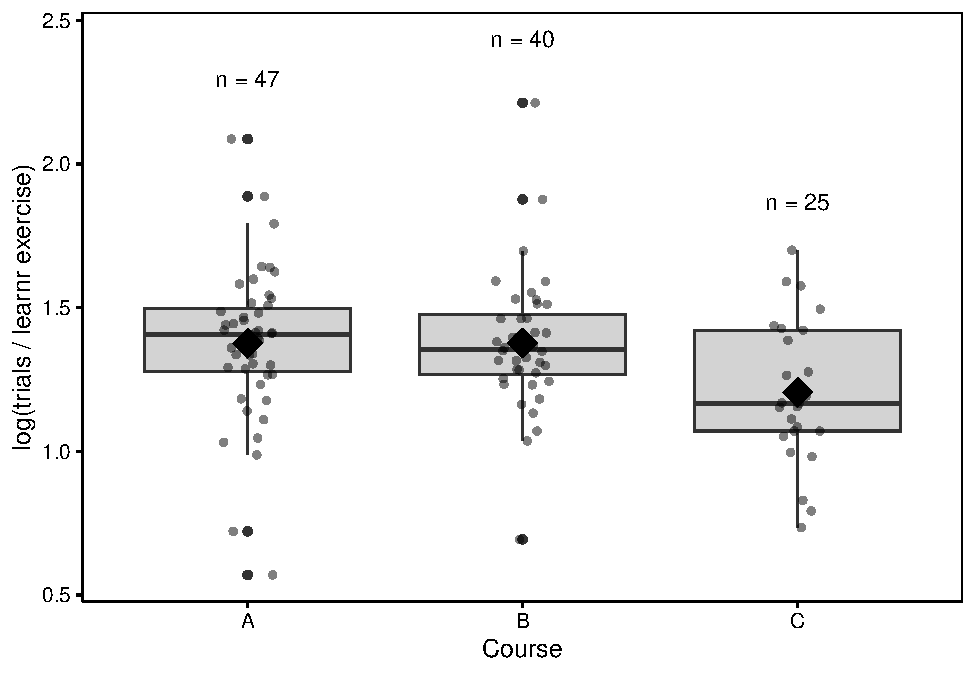
\includegraphics{teaching_data_science_files/figure-latex/fig_learn_trials-1.pdf}
\caption{\label{fig:fig_learn_trials} Average number of retries that
where required for each student to find the right answer in learnr
tutorials exercises (year 2020-2021). This measure is used as an
indirect, but objective measurement of the cognitive workload. The black
dot is the average for the whole classes and \emph{n} is the number of
observations.}
\end{figure}

The objective measurement of the cognitive workload based on the average
number of entries that where required for each student to find the right
answer in learnr tutorials exercises (Fig. \ref{fig:fig_learn_trials} ).
This indirect measure varies significantly between the 3 courses (ANOVA,
F(2,109) = 3.655, p-value = 0.029). The students in course C need
significantly fewer trials to find the right answer than students in
courses A (Tukey HSD, t = -2.489, p-value = 0.0375) and B (Tukey HSD, t
= 0.0474, p-value = 0.047)

The perceived cognitive load required to perform these exercises is also
a key aspect. This measure the emotional state of the students after
having completed a tutorial. This has, as far as we know, not been
studied yet. We used a NASA LTX questionnaire to assess it across all
three courses. Participation to the survey was high: 48/59 (81\%), 35/45
(78\%) and 18/26 (69\%) for courses A, B, and C respectively.

\begin{figure}
\centering
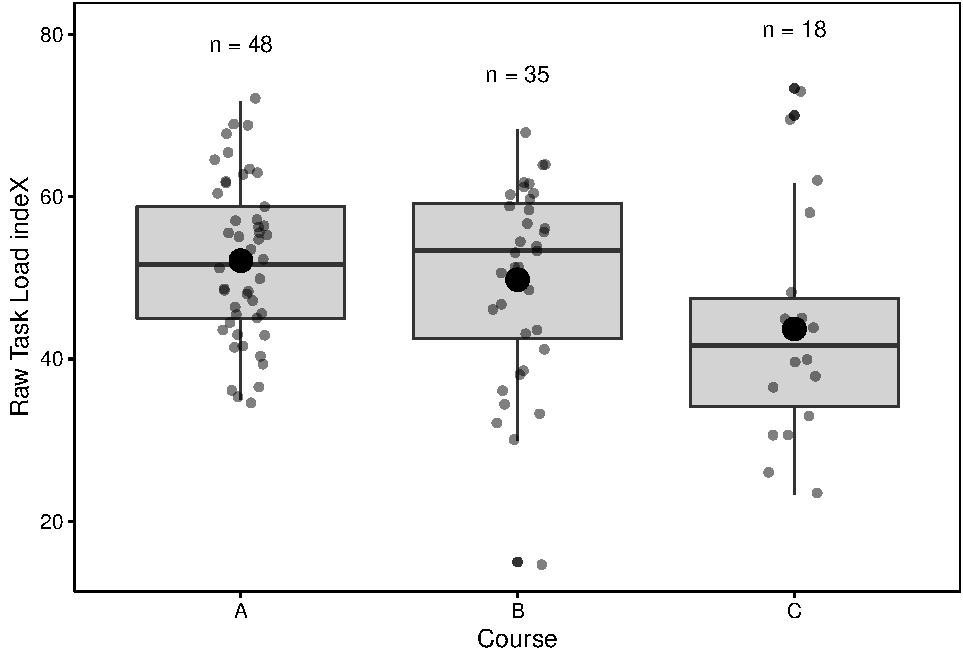
\includegraphics{teaching_data_science_files/figure-latex/fig_rtlx-1.pdf}
\caption{\label{fig:fig_rtlx} Perceived workload for the learnr
tutorials in the three courses (year 2020-2021). The black circle is the
mean RTLX value. The number above each box is the number of
respondants.}
\end{figure}

The difficulty of the course, and thus, of the exercises in the
tutorials increase from one course to the other. However, we do not
observe an increase, neither in the number of retries, nor in the RTLX
index (Fig. \ref{fig:fig_rtlx} ). On the contrary, these appear
significantly lower for course C than for course A (ANOVA, F(2,98) =
3.588, p-value = 0.031; Tukey HSD, t = -2.679, p-value = 0.023). The
cognitive load perceived by the students diminishes at the same time
their ability to find the right answer more rapidly. This may be a
consequence of a more fluent R coding and a better mastering of the
software environment.

\hypertarget{final-exam-versus-project}{%
\subsection{\texorpdfstring{Final exam \emph{versus}
project}{Final exam versus project}}\label{final-exam-versus-project}}

\begin{figure}
\centering
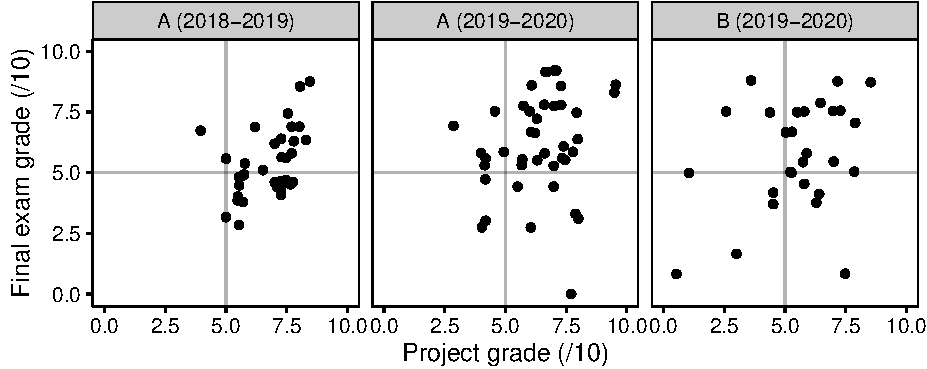
\includegraphics{teaching_data_science_files/figure-latex/fig_exams_projects-1.pdf}
\caption{\label{fig:fig_exams_projects} Grades obtained at the final
exam in function of grades obtained for the projects for courses A and B
during two years (course B was still in its old form in 2018-2019 and is
thus not represented).}
\end{figure}

In 2018-2019 and 2019-2020, the summative assessment was based on the
completion of a project and on a more conventional examination at the
end of the term. The comparison of the grades obtained by each student
for a project and a final exam shows only a weak correlation between
these two types of evaluations {[}TODO: provide values here{]}. Year
2018-2019 marks the transition to a flipped classroom approach in our
teaching of these data science courses. Only one student failed in the
project, while almost one third of the same students failed their final
exams. The difficulty of the project was similar to previous years, when
the course was made of lectures followed by exercises (and when failure
was not uncommon). The flipped classroom approach leaves more time in
class to work on practical applications, to ask questions, to discuss
results, \ldots{} We hypothesize that the very low failure rate could be
explained by a better preparation to practical data analysis, but not to
the final exam.

In 2019-2020, we raised a little bit the difficulty for the project,
resulting in a more widespread distribution of the results, but with a
similar pattern showing very little correlation between the two
evaluation methods. The same conclusion can be drawn for course B, with
several students failing in one of the two evaluations, but not in the
other one.

Despite, a final examination that includes a series of practical
questions (writing R code to analyse data, as in the projects), this
type of assessment does not reflect the ability of the students to
correctly process and analyse biological data. Alignment with intended
learning outcomes seem thus to be more present in the projects. Due to
these results, the final examination was abandoned for the year
2020-2021, and it has been replaced by a continuous evaluation of the
students' activities across all four level exercises. These activities
are analysed in the following section.

\hypertarget{students-activity-profiles-in-continuous-evaluation}{%
\subsection{Students activity profiles in continuous
evaluation}\label{students-activity-profiles-in-continuous-evaluation}}

In 2020-2021, to support the continuous evaluation method without final
exam, the course material was enriched with exercises organized into
four increasing difficulty levels, as presented in Table XXX. The
activity of the students in level 1 (H5P) and 2 (learnr) exercises is
directly recorded in a database. For the GitHub projects (levels 3 and 4
exercises), it is the git log data that are analysed. During lockdown
periods, exchange with students and answers to their questions were
exclusively done by email, text or voice messages on Discord, either on
private or public channels. Students were allowed to freely chose their
favourite way to interact with the teachers and between each other. All
these exchanges were recorded too. Finally, records in all activities
were used to establish the final grade for the course.

Final grade is the weighted average of the scores obtained at all four
levels. The weight was adjusted from course to course according to the
importance of the different projects, mainly. To give an idea, for
course A second term, level 1 H5P exercises accounted for 5\%, 10\% for
level 2 learnr tutorials, 35\% for level 3 individual projects and 40\%
for level 4 group works. More weight is always put on projects. On
average, each student went thorugh more than 130 assessments that
accounted for the final grade. Two third of these assessments were
established manually, using evaluation grids based on the reports they
write using R Markdown {[}TODO: add a ref here{]} (.Rmd files, a
literate programming system that allows to include computations directly
inside the report) in their projects. The remaing third is made of
scores automatically calculated from the various online exercises.

For the three courses, we recorded a total of more than 450,000 events,
which makes on average almost 3,500 events for each student. These data
contain information to characterize the behaviour and learning patterns
that the students use. They are summarized into sixteen metrics.

For H5P exercises:

\begin{itemize}
\tightlist
\item
  trials/H5P ex.: the average number of trials for each H5P exercise
  (students can retry as much as they wish and they have immediate
  feedback if their answer is correct or not),
\item
  correct H5P ex.: the fraction of H5P exercises that were correctly
  answered,
\end{itemize}

For learnr tutorial exercises:

\begin{itemize}
\tightlist
\item
  trials/learnr ex.: the average number of trials for each learnr
  exercise (here also, students can retry as much as they want),
\item
  hints/learnr ex.: in learnr exercises, students can display hints to
  help them to solve the problems (but they lose 10\% of the score of
  the exercise for each hint they view). This is the average number of
  hints per exercise that were displayed,
\item
  correct learnr ex.: the fraction of learnr exercises that were
  completed with a correct answer,
\item
  time/learnr ex.: the average time required to finish one learnr
  exercise involving R code writing.
\end{itemize}

For individual and group projects:

\begin{itemize}
\tightlist
\item
  commits/ind. projects: the average number of commits done by a student
  in one individual project,
\item
  contributions/ind. projects: the number of lines changed (added or
  subtracted) in an R Markdown report by one student in one individual
  project, on average,
\item
  commits/group projects: same as above, but for group projects,
\item
  contributions/group projects: same as above, but for group projects,
\item
  percentage of contribution to group projects: the fraction of work the
  student did, relative to all the work done in group projects (still
  only counted for .Rmd files as the number of lines changed from one
  version to the other).
\end{itemize}

For support:

\begin{itemize}
\tightlist
\item
  questions/module: the number of questions student asked in total,
  divided by the number of modules in the course,
\item
  percent of public question: the fraction of questions that the student
  posted in a public channel (a channel dedicated to the course that all
  the other students of the class can read),
\item
  contributions/question: a metric that catches the relative
  ``productivity'' of the student related to the number of questions
  they ask.
\end{itemize}

Finally, global measurements:

\begin{itemize}
\tightlist
\item
  work done: the fraction of all exercises that the student finished,
\item
  work done in time: the fraction the the exercises done in the right
  time, that is, during the proposed calendar.
\end{itemize}

In our courses, we have a few students in mobility that come from
various origins. The a priori knowledge is important in education. So,
to avoid biases due to the past curriculum of the students, we restrict
this analysis to the subpopulation that comes from the first year of
Bachelor in Biology at UMONS only. A Kohonen's self-organizing map is
used to create student profiles according to their activities, see Fig.
XXX. A 3x3 hexagonal cells pattern was chosen, and students are thus
classified into nine different classes.

\begin{figure}
\centering
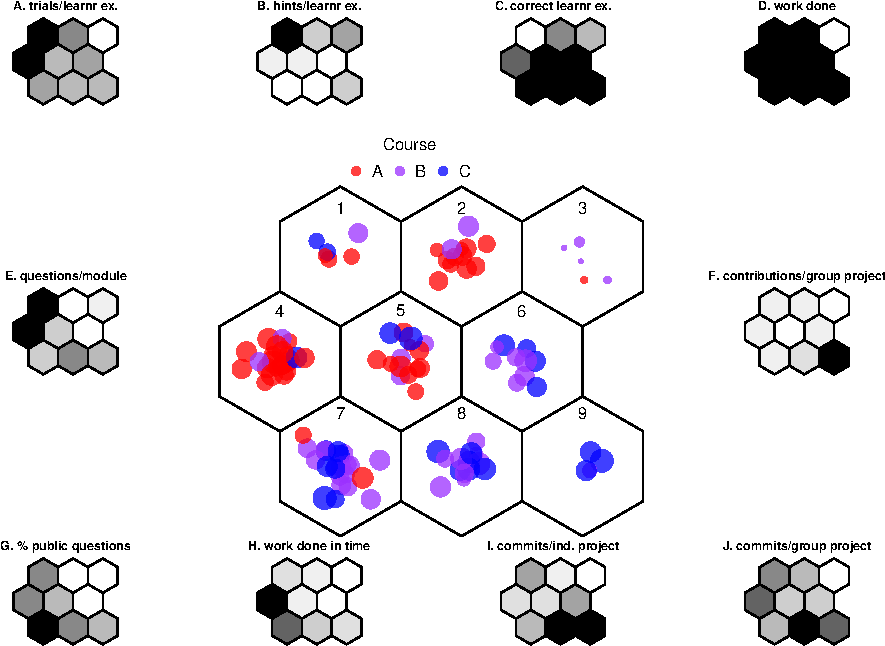
\includegraphics{teaching_data_science_files/figure-latex/fig_som-1.pdf}
\caption{\label{fig:fig_som} Self-organizing map of the student
activities across the three courses (year 2020-2021). See the text for
the explanations.}
\end{figure}

In \ref{fig:fig_som}, the small plots in gray show how selected metrics
distribute in the nine cells, from lowest value in white to highest
value in black. They help to decrypt the way students behave according
to their profile. Metrics that are not represented present similar
patterns than others (for instance H5P metrics exhibit a similar pattern
as learnr metrics and therefore, they are not represented). Dots in the
central plot are the various students, with colour representing the
course and the diameter of the dots representing the grade the students
obtained at the end of the course. The following paragraphs detail
information in that figure. The numbers between brackets mean the cell
number in the central plot, and the upper case letters in brackets refer
to the peripheral sub-plots.

Although most students finished all, or almost all exercises (D), cell
(3) collects the few student that did only a very small part of the
exercises. These students obtained very low grades, of course. They
belong to courses A and B. On the other hand, heavy workers are at the
bottom (I \& J), and good performers in learnrs (C) are in cells (5-9).

\begin{itemize}
\item
  Besides the absent students of cell (3), cells (2 and 6) collect
  students that seldom ask questions (E), and that rarely appear on the
  public channel (G). Minor differences separate them. For instance,
  cell (2) sometimes use learnr hints (B), while cell (6) never does,
  also because they find the correct answer to the exercises more often
  by themselves (C). Asking questions is at the core of our pedagogical
  approach. So, these students do not play the game. However, they can
  possibly succeed. Some of them probably exchange with other students
  through different channels that we do not monitor. It is interesting
  to note that the cell (2) -more difficulties with learnr tutorials-
  are mainly students of course A, while cell (6) contains students of
  courses B and C. There is a clear evolution in their behaviour from
  one course to the other in term of ease in front of the exercises,
  even if they remain silent in term of teacher interactions.
\item
  Among the students that have hard time to figure out the answers to
  auto-evaluation exercises, cell (1) reassemble people that most
  heavily rely on learnr hints (B), and also are among those who need to
  retry those exercises more often before figuring out the correct
  answer (A), a characteristic they share with cell (4). These students
  also ask a lot of questions (E), both on the public and private
  channels (G, mid gray). Main difference between those two groups is
  that students in cell (4) try harder to find the answer without
  looking at the hints, while in cell (1) they give up more rapidly.
  Also these students respect the proposed schedule much more closely
  than all others (H). We have students in all courses there, but a
  majority from course A.
\item
  All these cells (1-4 plus 6) are students that exhibits sub-optimal
  behaviours in one or the other way. The remaining cells (5 \& 7-9)
  correspond to students that perform better from this point of view.
  Cell (5) has a majority of people from course A, but otherwise, also
  from course B and C. These are average actors in all categories,
  except they are fluent with level 1 (H5P, not shown) and level 2
  (learnr, C) exercises.
\item
  Moving from cell (5) to (7), (8) and (9), we encounter increasingly
  top performers. The number of students from course A becomes
  progressively lower, while course B, and especially C dominate in
  these groups. Cell (7) use largely the public channel (G) and respect
  the schedule quite well (H) as main difference from those from cell
  (5). Students in cells (8) and (9) are not so much in time, but this
  is because they are heavier workers in the projects, both in the
  individuals (I) and in the groups (J) activities. This needs obviously
  more time. In cell (9) we have also the students that contributes the
  most to the reports in term of lines added or deleted (F).
\end{itemize}

In overall, at the top of the SOM, cells (1-4, plus 6) contain students
with not optimal behaviour, cell (5) are average students, and cells
(7-9) at the bottom exhibit profiles corresponding to best performers.
The pattern is also visible between courses A (mainly distributed at the
top or centre) to B and C (more represented at the bottom). This
suggests that students need time to get used to the course, its
pedagogical approach, and/or the software environment they have to use.

\hypertarget{transition-between-face-to-face-and-distance-learning}{%
\subsection{Transition between face-to-face and distance
learning}\label{transition-between-face-to-face-and-distance-learning}}

Due to Covid-19 lockdown periods, distance learning had to be adopted
abruptly. We analyse the activity collected during academic years
2019-2020 and 2020-2021 to evaluate the impact of these transition on
the progression of the students In Fig. XXX, the academic term is
divided here into seven work periods of approximately two weeks (remind
that it is the rhythm of the courses: one module every second week). The
classes of the second term of the year 2019-2020 start at period Y1P09,
since period Y1P08 is reserved for the exams. The courses of the first
term of 2020-2021 begins at Y2P01. First lockdown started at period
Y1P11 for one month and an half. Second lockdown stared at Y2P03 and
lasted at then end of the second term (Y2P15). During the first
lockdown, we rapidly opened the dedicated Discord channels and a common
email address for all teachers was installed for a faster reaction.

\begin{figure}
\centering
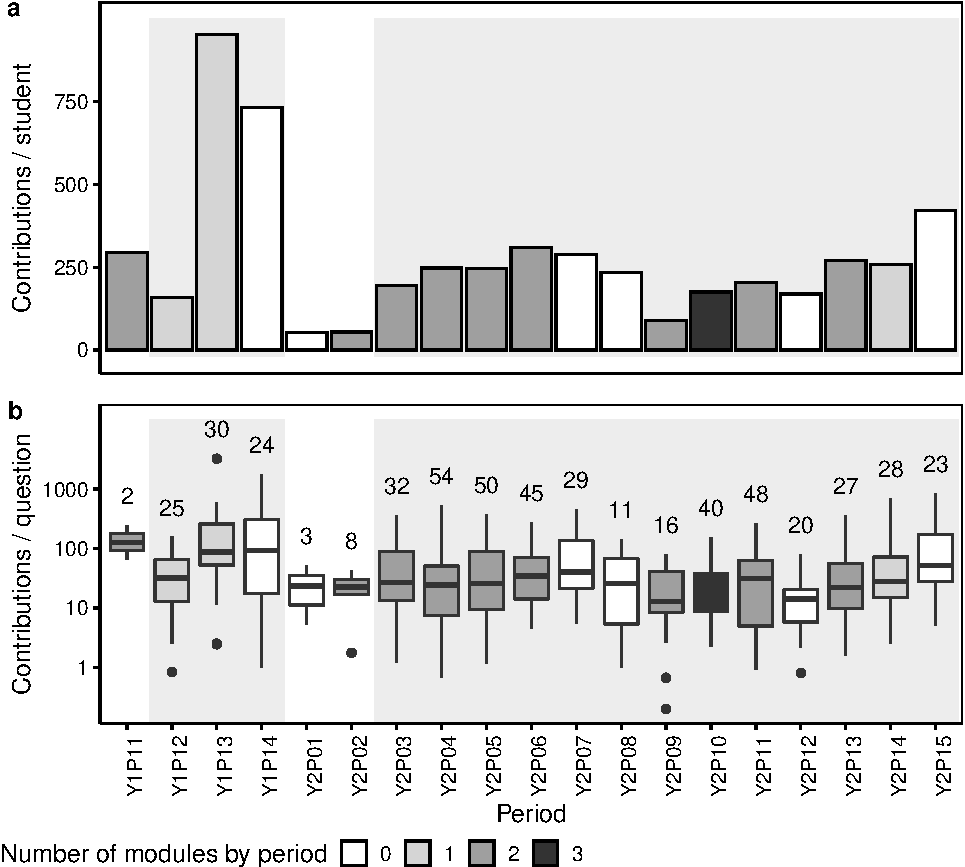
\includegraphics{teaching_data_science_files/figure-latex/fig_support_by_time-1.pdf}
\caption{\label{fig:fig_support_by_time} a. Contributions of the
students to the projects by periods of two weeks of course. b.
Contributions by question asked (log scale) as a proxy measurement of
the effect of student-teacher interactions on the progression in data
analysis. Light gray background indicates periods where distance
teaching was mandatory due to Covid-19 lockdown (Y1 is 2019-2020, Y2 is
2020-2021).}
\end{figure}

{[}TODO: this paragraph must be adapted and reworked!{]} The
contributions to the reports remains relatively proportional to the
number of questions the students sent by email or Discord messages, no
matter the period and the intensity of the work as indicated by the
number of modules to be completed during the period, all three courses
pooled together. Only the number of students that ask questions by there
channels change between face-to-face and distance teaching (much less in
face-to-face because most of the students ask their questions directly
in the classroom). Transition from direct interaction to electronic
exchange was quasi immediate during lockdown. Consequently, support
provided by the teachers in distance learning \ldots{} to be continued.

\hypertarget{discussion}{%
\section{Discussion}\label{discussion}}

Teaching data science to a population of students that are not very used
to advanced computer techniques and tools, and that have only basic
knowledge in mathematics and statistics is a hard task {[}18{]}. Our
basic approach is to extend the training on a very long period: five
successive terms spanning on three consecutive years (undergraduate and
graduate). That way, the many different concepts they have to learn can
be break down into subunits (26 modules) that last for two week each. We
also used flipped classrooms and blended course, with an emphasis on
proactive exchange with the teachers: students have to ask questions to
progress.

Our students are more used to a traditional approach made of lectures
followed by exercises where important concepts are repeated at the
beginning of the practical sessions. They tend to have a passive
attitude during lectures and they expect the teachers and assistants
literally feed them with the key concepts. That attitude does not work
here. Proactivity and autonomy is required {[}14{]}. They have thus to
learn a very different way of learning. The transition between the
theory they read in the book and the projects where they have to apply
these concepts is too abrupt without a progression in three stages
essentially: (1) auto-evaluation exercises directly in the book, (2)
recall of the main concepts and guided step-by-step analysis of a first
dataset with the learnr tutorials and (3) at least one guided individual
project with another dataset. The middle task, the learnr tutorial, was
immediately spotted by our students as a key activity in 2018-2019. So,
we have focused our attention on these documents in the following years.
In 2020-2021, we have also tested the addition of an heuristic engine
(gradethis) to provide contextual feedback on the errors students make
in their answers. The RTLX index measured in 2020-2021 will serve in the
future as reference to work towards correctly designed tutorials, with
lower perceived workload without sacrificing the content. The
significant decrease in RTLX value from course A to C indicates that
there a still a margin of progression. We would like to see this
decrease sooner, perhaps already in the second course.

Ultimately, the task that better evaluates their practical skills in
biological data analysis is the group project because they have to
demonstrate what they can do with a dataset and minimal instructions.
They have to figure out a suitable question, analyse the data to answer
that question, present their results in a report and discuss what they
found with a critical mind {[}13{]}. This task is complex, especially
for undergraduate students. That is why it is run in groups of two to
four students, depending on the complexity of the problem. Here, they
mobilize their collective intelligence to get results many of them would
be hardly capable to achieve alone. Yet, the tracking of individual
activity in the project through git allows to figure out clearly what
was the contribution of each student in the group and to score their
individual contributions in a suitable way.

Sometimes, groups do not work well, and one student has to do most of
the work. This is a clear weakness in this approach, especially if one
of the students in Fig. \ref{fig:fig_som} cell (3) is involved. If we
could identify the profile of the different students relatively early
during the course, we would be able to create better grouping with a
blend of different complimentary profiles in order to enrich their
experience. May be should we work exclusively with groups of four
students to mitigate the impact of one student that does not its job?

Those group projects are also key activities to evaluate the competences
of ours students. We observed a very low correlation between
performances in projects and grading obtained at final exams. This led
us to stop final exams, at the benefit of a continuous evaluation with
highest weight in the final grade for group projects (Fig.
\ref{fig:fig_exams_projects} ). It requires to set up a system to
monitor and score the students' activity in all the exercises, either by
automatic scoring of online exercises, or by using an evaluation grid
for manual assessment of their projects. This is time-consuming but the
partial automatic scoring lowers the charge. It would be interesting to
design tools that could second teachers in these assessments. For
instance, reproducible research is one of the competences our students
have to develop. This implies that their R Markdown documents should
compile into reports in HTML or PDF format without any error. This
criterion could be checked automatically.

Activity tracking in the exercises, primarily set up for the continuous
evaluation, offers also the possibility to study the way student
progress in the material. Classification of the students according to
their behaviour is an interesting approach. It paves the way toward a
more inclusive pedagogy by spotting different kinds of sub-optimal
behaviours (not asking questions, looking at hints without searching
much by oneself the answer, being shy to discuss problems on public
channels, \ldots) Once these sub-optimal patterns are evidenced, we can
think of counter-measures. For instance, we will test public channels
were teachers never post. However, they can read the discussions between
students. In case of errors, the teacher contact the student privately
to explain what is wrong. Then that student would have to come back with
a correction. Their error is thus not publicly spotted by the teacher,
and the student has the resposibility to reexplain to its siblings. This
approach was very successful with our ``eleve-assitants'' (students from
higher classes that have brilliantly succeeded in the course one or two
years before and that second the teachers).

With tools like the self-organizing map, we should be able to predict
student profiles early during the courses in order to spot the
problematic patterns much faster. That way, we could engage specific
discussions with the concerned students to determine the cause of the
problems and try to solve them before it is too late. With this tool, we
certainly enter in a differential pedagogical approach, which is one key
to more inclusive teaching {[}ref needed here{]}. Emotional state of the
students and motivation are also very important. Validated
questionnaires, like NASA-LTX, or {[}\ldots.complete here{]} allow us to
assess these aspect.

{[}I still have to write a paragraph that discusses the results
regarding the timing events around covid-19 lockdown periods and their
implications\ldots.{]}

\hypertarget{conclusion}{%
\section{Conclusion}\label{conclusion}}

Teaching data science comes with specific challenges. The discipline is
quite young and we still are seeking the best pedagogical approach.
After three years of teaching data science to undergraduate and graduate
students in a cursus in biology with revised pedagogical practices, we
have our first cohort that has followed all three courses. There are
still two optional courses in second Master if they want to push their
data science skills further on. However, these three courses are
designed to be sufficient by themselves. Globally, most students
acquired the competences during these courses. We have the feeling that
they are more mature and more capable in data science than with our
previous courses in biostatistics given in a more traditional way. The
impact of the revised approach to biological data science on the way
learners manage data and data analysis will be observable during the
following years. We will observe how these students apply their skills
in their master thesis, and later, in their career or during their PhD
thesis. In the meantime, we will continue to improve our courses by
further exploiting the data we accumulated on the student activities.
Experience gathered during forced distance learning during Covid-19
lockdown will be used too to improve our courses. The radical changes
that were required in that particular context showed that students can
accomodate to a large extent, but also that a diversification of the
activities is beneficial {[}citer Spadofora et Marini 2018{]}. Speaking
about diversification, we have succesfully tested in 2020-2021 a
kaggle-like challenge (\url{https://www.kaggle.com/competitions}) in one
of the machine learning modules. Such more ludic activities would also
contribute to the diversification of pedagogical practices, interest and
motivation of the students {[}refs needed if possible{]}. We would also
be happy to share experience with other teachers in data science. All
together, we are asked to shape the post-covid teaching landscape, and
it will probably be quite different to what we are using today!

\hypertarget{references}{%
\section*{References}\label{references}}
\addcontentsline{toc}{section}{References}

\hypertarget{refs}{}
\begin{CSLReferences}{0}{0}
\leavevmode\hypertarget{ref-Marx2013}{}%
\CSLLeftMargin{1. }
\CSLRightInline{Marx V (2013) {The big challenges of big data}.
\emph{Nature} 498: 255--260.}

\leavevmode\hypertarget{ref-Baker2016}{}%
\CSLLeftMargin{2. }
\CSLRightInline{Baker M (2016) 1,500 scientists lift the lid on
reproducibility. \emph{Nature} 533: 452--454.}

\leavevmode\hypertarget{ref-Banks2019}{}%
\CSLLeftMargin{3. }
\CSLRightInline{Banks GC, Field JG, Oswald FL, et al. (2019) {Answers to
18 Questions About Open Science Practices}. \emph{Journal of Business
and Psychology} 34: 257--270.}

\leavevmode\hypertarget{ref-Donoho2017}{}%
\CSLLeftMargin{4. }
\CSLRightInline{Donoho D (2017) {50 Years of Data Science}.
\emph{Journal of Computational and Graphical Statistics} 26: 745--766.}

\leavevmode\hypertarget{ref-Cetinkaya-Rundel2021}{}%
\CSLLeftMargin{5. }
\CSLRightInline{Çetinkaya-Rundel M, Ellison V (2021) {A Fresh Look at
Introductory Data Science}. \emph{Journal of Statistics Education} 0:
1--27.}

\leavevmode\hypertarget{ref-Onwuegbuzie2003}{}%
\CSLLeftMargin{6. }
\CSLRightInline{Onwuegbuzie AJ, Wilson VA (2003) {Statistics Anxiety:
Nature, etiology, antecedents, effects, and treatments--a comprehensive
review of the literature}. \emph{Teaching in Higher Education} 8:
195--209.}

\leavevmode\hypertarget{ref-Fiksel2019}{}%
\CSLLeftMargin{7. }
\CSLRightInline{Fiksel J, Jager LR, Hardin JSJS, et al. (2019) {Using
GitHub Classroom To Teach Statistics}. \emph{Journal of Statistics
Education} 27: 110--119.}

\leavevmode\hypertarget{ref-Hsing2019}{}%
\CSLLeftMargin{8. }
\CSLRightInline{Hsing C, Gennarelli V (2019) {Using GitHub in the
Classroom Predicts Student Learning Outcomes and Classroom Experiences:
Findings from a Survey of Students and Teachers}, \emph{Proceedings of
the 50th ACM technical symposium on computer science education}, New
York, NY, USA, Association for Computing Machinery, 672--678.}

\leavevmode\hypertarget{ref-Baumer2014}{}%
\CSLLeftMargin{9. }
\CSLRightInline{Baumer B, Cetinkaya-Rundel M, Bray A, et al. (2014) {R
Markdown: Integrating A Reproducible Analysis Tool into Introductory
Statistics}. \emph{Technology Innovations in Statistics Education} 8.}

\leavevmode\hypertarget{ref-Cetinkaya-Rundel2018}{}%
\CSLLeftMargin{10. }
\CSLRightInline{Çetinkaya-Rundel M, Rundel C (2018) {Infrastructure and
Tools for Teaching Computing Throughout the Statistical Curriculum}.
\emph{American Statistician} 72: 58--65.}

\leavevmode\hypertarget{ref-Boettiger2015}{}%
\CSLLeftMargin{11. }
\CSLRightInline{Boettiger C (2015) {An Introduction to Docker for
Reproducible Research}. \emph{SIGOPS Oper Syst Rev} 49: 71--79.}

\leavevmode\hypertarget{ref-Larwin2011}{}%
\CSLLeftMargin{12. }
\CSLRightInline{Larwin K, Larwin D (2011) {A meta-analysis examining the
impact of computer-assisted instruction on postsecondary statistics
education: 40 years of research}. \emph{Journal of Research on
Technology in Education} 43: 253--278.}

\leavevmode\hypertarget{ref-Auker2020}{}%
\CSLLeftMargin{13. }
\CSLRightInline{Auker LA, Barthelmess EL (2020) {Teaching R in the
undergraduate ecology classroom: approaches, lessons learned, and
recommendations}. \emph{Ecosphere} 11: e03060.}

\leavevmode\hypertarget{ref-Freeman2014}{}%
\CSLLeftMargin{14. }
\CSLRightInline{Freeman S, Eddy SL, McDonough M, et al. (2014) {Active
learning increases student performance in science, engineering, and
mathematics}. \emph{Proceedings of the National Academy of Sciences}
111: 8410--8415.}

\leavevmode\hypertarget{ref-Estrellado2020}{}%
\CSLLeftMargin{15. }
\CSLRightInline{Estrellado RA, Bovee EA, Mostipak J, et al. (2020) {Data
science in education using R}, London, England, Routledge.}

\leavevmode\hypertarget{ref-Hart1988}{}%
\CSLLeftMargin{16. }
\CSLRightInline{Hart SG, Staveland LE (1988) {Development of NASA-TLX
(Task Load Index): Results of Empirical and Theoretical Research}.
\emph{Advances in Psychology} 52: 139--183.}

\leavevmode\hypertarget{ref-Byers1989}{}%
\CSLLeftMargin{17. }
\CSLRightInline{Byers JC, Bittner A, Hill S (1989) {Traditional and raw
task load index (TLX) correlations: Are paired comparisons necessary? In
A}.}

\leavevmode\hypertarget{ref-Sousa2018}{}%
\CSLLeftMargin{18. }
\CSLRightInline{Sousa D, Sorto IMA, White A (2018) {Teaching With R---A
Curse or a Blessing?}, \emph{Looking back, looking forward. Proceedings
of the tenth international conference on teaching statistics}, Kyoto,
International Statistical Institute.}

\end{CSLReferences}

\end{document}
